\chapter{Dual Spaces}

\section{Quotient Spaces}

Let $S$ be a subspace of a vector space $V$. Recalling the modular arithmetic, it is easy to see that the binary relation on $V$ defined binary
\[
	u \equiv v \iff u-v \in S
\]
is an equivalence relation. We say that $u$ and $v$ are \textbf{congruent modulo $S$}.

Now notice that
\begin{equation*}
	\begin{aligned}
		[v] &= \{ u \in V : u \equiv v \} \\
			&= \{ u \in V : u-v \in S \} \\
			&= \{ u \in V : u = v+s, \text{ for some } s \in S \} \\
			&= \{ v + s : s \in S \} \\
			&= v + S
	\end{aligned}
\end{equation*}

The set
\[
	[v] = v + S = \{ v+s : s \in S \}
\]
is called a \textbf{coset} or \textbf{affine subset} of $S$ in $V$.

\begin{example}
	The solution set of a linear system 
	\[
		C = \{ x : Ax = b \}
	\]
	is an affine subspace, with $A \in \textbf{R}^{m \times n}$ and $b \in \textbf{R}^m$.
\end{example}

\begin{definition}[Quotient Space]
	The set of all cosets (or classes) of $S$ in $V$, denoted by
\[
	V / S = \{ v+s : v \in V \}
\]
is called the \textbf{quotient space of $V$ modulo $S$}.
\end{definition}

Naturally, we define addition and scalar multiplication as follows
\[
	(u + S) + (v + S) = (u + v) + S \text{ and } \lambda(u+S) = \lambda u + S
\]
which are well defined.

\begin{theorem}
	The quotient space of $V$ modulo $S$ is a vector space over $\textbf{F}$ with the operations
	\[
		\lambda(u + S) = \lambda u + S
	\]
	\[
		(u + S) + (v + S) = (u + v) + S
	\]
\end{theorem}

\begin{definition}[Natural Projection]
	If $S$ is a subspace of $V$, we may define the mapping 
	\[
		\pi_S : V \longrightarrow V/S
	\]
	which sends every vector to the coset containing it, i.e., the class associated to it. This map is called the \textbf{natural projection} or \textbf{canonical projection}.
\end{definition}

\begin{theorem}
	The canonical projection $\pi_S$ is a surjective linear mapping with $\ker (\pi_S) = S$.
\end{theorem}

\begin{theorem}[The Correspondence Theorem]
	Let $S$ be a subspace of $V$. Then the function that assigns each subspace $S \subset T \subset V$, the subspace $T/S$ of $V/S$ is an order-preserving one-to-one correspondence between the set of all subspaces of $V$ containing $S$ and the set of all subspaces of $V/S$.
\end{theorem}

\begin{figure}[h]
	\centering
	  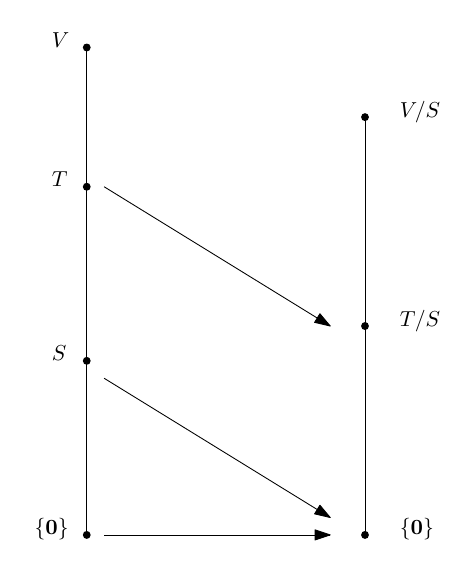
\includegraphics[width=0.37\textwidth]{Figures/correspondence_theorem.png} 
	  \caption{Correspondence between $V$ and $V/S$.}
	  \label{fig:correspondence-theorem}
\end{figure}

\begin{definition}[Codimension]
	Let $W$ be a subspace of $V$. Then the \textbf{codimension} of $W$ in $V$ is
	\[
		\text{codim}_V W = \dim V/W
	\]
\end{definition}

\begin{theorem}
	Suppose $\dim V = n$ and $W$ is a subspace of $V$ with $\dim W = k$. Then 
	\[
		\dim V/W = \text{codim}_V W = n-k
	\]
\end{theorem}

\begin{definition}[Cokernel and Coimage]
	Let $T : V \longrightarrow W$ a linear transformation. Then the \textbf{cokernel} of $T$ is the quotient space
	\[
		\text{coker} (T) = W / \text{Im}(T)
	\] 

	And the \textbf{coimage} of $T$ is defined as
	\[
		\text{coim} (T) = V / \text{Ker}(T)
	\]
\end{definition}

\begin{corollary}
	Let $V$ be a finite-dimensional vector space $T : V \longrightarrow V$ a linear transformation. Then 
	\[
		\dim (\ker (T)) = \dim (\text{coker} (T))
	\]
\end{corollary}

\section{Dual Space}

A concept that will help us in the study of subspaces, linear equations, and coordinates is the following.

\begin{definition}[Linear Functional and Dual Space]
	A linear transformation from the vector space $V$ to its scalar field $\textbf{F}$ is called a \textbf{linear functional}.
	
	The set of linear functionals is denoted by $V^\ast$ and is called \textbf{dual space} of $V$. In other words, $V^\ast = \mathcal{L}(V, \textbf{F})$.
\end{definition}

Linear functionals are also called a \textbf{form} or a \textbf{1-form}.

\begin{example}
	Let $(c_1, \ldots, c_n) \in \textbf{F}^n$ and define $f : \textbf{F}^n \longrightarrow \textbf{F}$ by 
	\[
		f(x_1, \ldots, x_n) = c_1 x_1 + \ldots + c_n x_n
	\]
	Then $f$ is a linear functional on $\textbf{F}^n$.
\end{example}

\begin{example}[Trace]
	If $A$ is an $n \times n$ matrix, the \textbf{trace} of $A$ is the scalar
	\[
		\text{tr } A = A_{11} + A_{22} + \ldots + A_{nn}
	\]
	
	Remark that the trace function is a linear functional on the matrix space $\textbf{M}_n$.
\end{example}

\begin{remark}
	Suppose $V$ is finite-dimensional. Then the dimension of the dual space is equal to the dimension of the space.
	\[
		\dim V^\ast = \dim V
	\]
\end{remark}

\begin{definition}[Dual basis]
	If $\beta = \{ v_1, \ldots, v_n \}$ is a basis of $V$ then the \textbf{dual basis} of $\beta$ is the set $\beta^\ast = \{ f_1, \ldots, f_n \}$, where each $f_i$ is the linear functional on $V$ such that 
	\[
		f_i(v_j) = \delta_{ij}
	\]
	where $\delta$ is the Kronecker's delta.
\end{definition}

\begin{theorem}
	Let $V$ be a finite-dimensional vector space. Then the dual basis of a basis of $V$ is a basis of $V^\ast$.
\end{theorem}

\begin{proof}
	Let $\beta = \{ v_1, \ldots, v_n \}$ be a basis for $V$. Then there exists a unique linear functional $f_i$ on $V$ such that
	\[
		f_i(v_j) = \delta_{ij}
	\]
	for each $i$.

	With this process, we obtain $n$ distinct linear functionals $f_1, \ldots, f_n$ on $V$.

	To show that $f_1, \ldots, f_n$ are linearly independent, suppose that $c_1, \ldots, c_n \in \textbf{F}$ are such that
	\[
		c_1 f_1 + \ldots + c_n f_n = 0
	\]
	Since $(c_1 f_1 + \ldots + c_n f_n)(v_j) = c_j$ for each $j = 1, \ldots, n$, we know that $c_1 = \ldots = c_n = 0$. Hence, $f_1, \ldots, f_n$ is linearly independent.
	
	And given that $\dim V^\ast = n$, the set $\beta^\ast = \{ f_1, \ldots, f_n \}$ is a basis for $V^\ast$.
\end{proof}

\begin{theorem}
	Let $\beta = \{ v_1, \ldots, v_n \}$ be a basis for a vector space $V$. Then there is a unique dual basis $\beta^\ast = \{ f_1, \ldots, f_n \}$ for $V^\ast$ such that $f_i (v_j) = \delta_{ij}$.
	
	For each linear functional $f$ on $V$ we have
	\[
		f = \sum_{i=1}^n f(v_i) f_i
	\]
	and for each vector $v \in V$ we have
	\[
		v = \sum_{i=1}^n f_i(v) v_i
	\]
\end{theorem}

\begin{proof}
	The last proof established that there is a unique basis which is `dual' to $\beta$. Let $f$ be a linear functional on $V$. Then $f$ is a linear combination of the $f_i$, so the scalars $c_j = f(v_j)$. Now, if
	\[
		v = \sum_{i=1}^n x_i v_i
	\]
	is a vector in $V$, then
	\[
		f_j(v) = \sum_{i=1}^n x_i f_j(v_i) = \sum_{i=1}^n x_i \delta_{ij} = x_j
	\]
	so $v$ has a unique expression as a linear combination of $v_i$ given by
	\[
		v = \sum_{i=1}^n f_i(v) v_i
	\]
\end{proof}

Note that $f_i$ are coordinate functions for $\beta$, given that $f_i$ assigns to each vector $v \in V$ the $i$th coordinate of $v$ relative to the ordered basis $\beta$.

How are linear functionals and subspaces related? If $f$ is a non-zero linear functional, then the rank of $f$ is one. And if $V$ is finite-dimensional, then by the \hyperref[thm:rank-null]{Rank–Nullity theorem}, the null space $N_f$ has dimension
\[
	\dim N_f = \dim V - 1
\]

In a vector space of dimension $n$, a subspace of of dimension $n-1$ is called a \textbf{hyperspace}, which is sometimes called \textbf{hyperplanes} or \textbf{subspaces of codimension one}. The hyperspace is always the null space of a linear functional.

\begin{definition}[Annihilator]
	Let $V$ be a vector space over $\textbf{F}$ and $S$ a subset of $V$. Then the \textbf{annihilator} of S is the set $S^0$ of linear functionals $f$ on $V$ such that $f(v) = 0$ for every $v \in S$.
	\[
		S^0 = \{ f \in V^\ast : f(v) = 0, \, \forall v \in S \}
	\]
\end{definition}

$S^0$ is a subspace of $V^\ast$. If $S = \{ 0 \}$, then $S^0 = V^\ast$. If $S = V$, then $S^0$ is the zero subspace of $V^\ast$.

The next example shows an important procedure in the following proofs.

\begin{example}
	Let $\{ e_1, e_2, e_3, e_4, e_5 \}$ be the standard basis of $\textbf{R}^5$ and $\{ f_1, f_2, f_3, f_4, f_5 \}$ be the dual basis of $\textbf{R}^5$. Suppose
	\[
		W = \text{span}(e_1, e_2) = \{ (x_1, x_2, 0, 0, 0)  \in \textbf{R}^5 : x_1, x_2 \in \textbf{R} \}
	\]
	We show that $W^0 = \text{span}(f_3, f_4, f_5)$.

	Recall that $f_j$ is the linear functional that selects the $j$th coordinate, i.e. $f_j(x_1, x_2, x_3, x_4, x_5) = x_j$.

	First suppose $f \in \text{span}(f_3, f_4, f_5)$. Then there exist $c_3, c_4, c_5 \in \textbf{R}$ such that $f = c_3 f_3 + c_4 f_4 + c_5 f_5$. If $(x_1, x_2, 0, 0, 0) \in W$, then 
	\[
		f(x_1, x_2, 0, 0, 0) = (c_3 f_3 + c_4 f_4 + c_5 f_5)(x_1, x_2, 0, 0, 0) = 0
	\]
	Hence $f \in W^0$. I.e., $\text{span}(f_3, f_4, f_5) \subset W^0$.

	Now suppose $f \in W^0$. Since the dual basis is a basis of $(\textbf{R}^5)^\ast$, there exist $c_1, \ldots, c_5 \in \textbf{R}$ such that $f = c_1 f_1 + c_2 f_2 + c_3 f_3 + c_4 f_4 + c_5 f_5$. Because $e_1 \in W$ and $f \in W^0$, we have
	\[
		0 = f(e_1) = (c_1 f_1 + c_2 f_2 + c_3 f_3 + c_4 f_4 + c_5 f_5)(e_1) = c_1
	\]

	Similarly, $e_2 \in W$ and thus $c_2 = 0$. Since $e_3, e_4, e_5 \notin W$, $f = c_3 f_3 + c_4 f_4 + c_5 f_5$. Thus $f \in \text{span}(f_3, f_4, f_5)$, i.e., $W^0 \subset \text{span}(f_3, f_4, f_5)$.
\end{example}

The next theorem states that each $d$-dimensional subspace of an $n$-dimensional space is the intersection of the null spaces of $(n-d)$ linear functionals.

\begin{theorem}\label{thm:dim-annihilator}
	Let $V$ be a finite-dimensional vector space and let $W$ be a subspace of $V$. Then
	\[
		\dim W + \dim W^0 = \dim V
	\]
\end{theorem}

\begin{proof}
	Let $\{ v_1, \ldots, v_k \}$ be a basis for $W$ and choose vectors $\{ v_{k+1}, \ldots, v_n \in V$ to extend to a basis $\{ v_1, \ldots, v_n \}$ of $V$. And let $ \{ f_1, \ldots, f_n \}$ be the basis for $V^\ast$ which is dual to this basis for $V$. We show that $\{ f_{k+1}, \ldots, f_n \}$ is a basis for $W^0$.

	For $i \geq k+1$, since $f_i(v_j) = \delta_{ij}$ and $\delta_{ij} = 0$ if $i \geq k+1$ and $j \leq k$, we know that $f_i$ belongs to $W^0$. Hence, for $i \geq k+1$,  $f_i(v) = 0$ whenever $v$ is a linear combination of $v_1, \ldots, v_k$.

	Given that the functionals $f_{k+1}, \ldots, f_n$ are linearly independent, all we need to show is that they span $W^\ast$. Suppose $f \in V^\ast$. Now 
	\[
		f = \sum_{i=1}^n f(v_i)f_i
	\]
	implies that if $f \in W^0$, we have $f(v_i) = 0$ for $i \leq k$ and
	\[
		f = \sum_{i = k+1}^n f(v_i) f_i
	\]

	Therefore, $W^0$ has dimension $n-k$, as desired.
\end{proof}

The next corollary shows that if we select some select ordered basis for the space, each $k$-dimensional subspace can be described by specifying $(n-k)$ homogeneous linear conditions on the coordinates relative to that basis.

\begin{corollary}
	If $W$ is a $k$-dimensional subspace of an $n$-dimensional vector space $V$, then $W$ is the intersection of $(n-k)$ hyperspaces in $V$.
\end{corollary}

\begin{corollary}\label{cor:determined-annihilator}
	If $W_1$ and $W_2$ are subspaces of a finite-dimensional vector space, then $W_1 = W_2$ iff. $W_1^0 = W_2^0$.
\end{corollary}

This theory provides a `dual' point of view on the system of equations, showing how annihilators are related to systems of homogeneous linear equations.

\begin{example}
	Let $W$ be the subspace of $\textbf{R}^5$ spanned by the vectors $v_1 = (2, -2, 3, 4, -1)$, $v_2 = (-1, 1, 2, 5, 2)$, $v_3 = (0, 0, -1, -2, 3)$, and $v_4 = (1, -1, 2, 3, 0)$.

	To find the annihilator $W^0$ of $W$, we first form a matrix $A$ with row vectors $v_1, v_2, v_3, v_4$ and find the row-reduced echelon matrix $R$ which is row-equivalent to $A$.
	\[
		A = \begin{bmatrix}
			2 && -2 && 3 && 4 && -1 \\
			-1 && 1 && 2 && 5 && 2 \\
			0 && 0 && -1 && -2 && 3 \\
			1 && -1 && 2 && 3 && 0
		\end{bmatrix}
		\longrightarrow
		R = \begin{bmatrix}
			1 && -1 && 0 && -1 && 0 \\
			0 && 0 && 1 && 2 && 0 \\
			0 && 0 && 0 && 0 && 1 \\
			0 && 0 && 0 && 0 && 0
		\end{bmatrix}
	\]

	Now, if $f$ is a linear functional on $\textbf{R}^5$, 
	\[
		f(x_1, \ldots, x_5) = \sum_{j=1}^5 c_j x_j
	\]
	and $f$ is in $W^0$ iff. $f(v_i) = 0$, for $i = 1,2,3,4$.
	
	This is equivalent to $Ac = 0$, where $c = (c_1, c_2, c_3, c_4, c_5)^t$. Which is, in turn, equivalent to $Rc = 0$. Or simply
	\begin{equation*}
		\begin{aligned}
			c_1 - c_2 - c_4 = 0 \\
			c_3 + 2 c_4 = 0 \\
			c_5 = 0
		\end{aligned}
	\end{equation*}

	By setting $c_2 = a$ and $c_4 = b$, we have $c_1 = a+b$, $c_3 = -2b$, $c_5 = 0$. So $W^0$ consists of all linear functionals of the form
	\[
		f(x_1, x_2, x_3, x_4, x_5) = (a+b)x_1 + ax_2 - 2bx_3 + bx_4
	\]

	The dimension of $W^0$ is two and a basis $\{ f_1, f_2 \}$ for it can be found by setting $a = 1, b = 0$, and then $a = 0, b = 1$:
	\begin{equation*}
		\begin{aligned}
			f_1(x_1, \ldots, x_5) &= x_1 + x_2 \\
			f_2(x_1, \ldots, x_5) &= x_1 - 2x_3 + x_4
	\end{aligned}
\end{equation*}
	And the general form of $f \in W^0$ is $f = a f_1 + bf_2$.
\end{example}

\section{The Double Dual}

Is every basis for $V^\ast$ the dual of some basis for $V$? To answer that question we consider $V^{\ast \ast}$, the dual space of $V^\ast$.
	
Let $v \in V$. Then $v$ \textbf{induces} a linear functional $L_v$ on $V^\ast$ defined by
\[
	L_v(f) = f(v), \, \text{ where } f \in V^\ast
\]
It is easy to check that $L_v$ is linear simply using the definition of linear operations in $V^\ast$.
\begin{equation*}
	\begin{aligned}
		L_v(cf + g) &= (cf+g)(v) = (cf)(v) + g(v) \\
					&= cf(v) + g(v) = cL_v(f) + L_v(g)
	\end{aligned}
\end{equation*}

\begin{theorem}
	Let $V$ be a finite-dimensional vector space. For each vector $v \in V$ define
	\[
		L_v(f) = f(v), \, \text{ where } f \in V^\ast
	\]
	The mapping $v \longrightarrow L_v$ is an isomorphism of $V$ onto $V^{\ast \ast}$.
\end{theorem}

\begin{proof}
	Suppose that $v, u \in V$ and $c \in \textbf{F}$ and let $w = cv + u$. Then for each $f \in V^\ast$,
	\begin{equation*}
		\begin{aligned}
			L_w(f) &= f(w) = f(cv + u) = cf(v) + f(u) \\
				   &= cL_v(f) + L_u(f)
		\end{aligned}
	\end{equation*}
	Hence, $v \longrightarrow L_v$ is a linear mapping from $V$ to $V^{\ast \ast}$.

	Notice that $L_v = 0$ iff. $v = 0$ by linearity, i.e., $L_v$ is a non-singular linear transformation.

	And given that 
	\[
		\dim V^{\ast \ast} = \dim V^\ast = \dim V
	\]
	we know that $L_v$ is bijective. Hence, this linear mapping is an isomorphism of $V$ onto $V^{\ast \ast}$.
\end{proof}

\begin{corollary}
	Let $V$ be a finite-dimensional vector space. If $L$ is a linear functional on the dual space $V^\ast$, then there is a unique vector $v \in V$ such that $L(f) = f(v)$, for every $f \in V^\ast$.
\end{corollary}

\begin{corollary}
	Let $V$ be a finite-dimensional vector space. Each basis for $V^\ast$ is the dual of some basis for $V$.
\end{corollary}

\begin{proof}
	Let $\beta^\ast = \{ f_1, \ldots, f_n \}$ be a basis for $V^\ast$. Then there exists a basis $\{ L_1, \ldots, L_n \}$ for $V^{\ast \ast}$ such that $L_i(f_j) = \delta_{ij}$.

	By the previous corollary, for each index $i$ there exists a vector $v_i \in V$ such that $L_i(f) = f(v_i)$, for every $f \in V^\ast$. Then $\{ v_1, \ldots, v_n \}$ is a basis for $V$ and $\beta^\ast$ is the dual of this basis.
\end{proof}

In this corollary we see that $V$ and $V^\ast$ are naturally in duality with one another. Each is the dual space of the other.

If $E$ is a subset of $V^\ast$, then the annihilator $E^0$ is a subset of $V^{\ast \ast}$. We know that each subspace $W$ is \hyperref[cor:determined-annihilator]{determined} by its annihilator $W^0$. This is the case because $W$ is the subspace annihilated by all $f \in W^0$, i.e., the intersection of the null spaces of all $f \in W^0$. We state this fact in the following identity
\[
	W = (W^0)^0
\]

\begin{theorem}
	If $S$ is any subset of a finite-dimensional vector space $V$, then $(S^0)^0$ is the subspace spanned by $S$.
\end{theorem}

\begin{proof}
	Let $W$ be the subspace generated by $S$. Clearly $W^0 = S^0$. We prove that $W = W^{00}$. By a \hyperref[thm:dim-annihilator]{previous theorem},
	\begin{equation*}
		\begin{aligned}
			\dim W + \dim W^0 &= \dim V \\
			\dim W^0 + \dim W^{00} &= \dim V^\ast
		\end{aligned}
	\end{equation*}
	
	Therefore, 
	\[
		\dim W = \dim W^{00}
	\]

	And since $W$ is a subspace of $W^{00}$, we have that $W = W^{00}$.
\end{proof}

The results of this section hold for arbitrary vector spaces using Axiom of Choice. In particular, we redefine \textbf{hyperspaces} in order to include the infinite dimensional case.

The idea is that a space $N$ falls just one dimension short of filling out $V$, using the concept of \hyperref[def:maximal]{maximal}.

\begin{definition}[Hyperspace]
	If $V$ is a vector space, a \textbf{hyperspace} in $V$ is a maximal proper subspace of $V$.
\end{definition}

Put another way, let $W$ be a proper subspace of $V$. If there isn't a subspace $U$ such that $W \subsetneq U \subsetneq V$, then $W$ is a hyperplane.

\begin{theorem}
	If $f$ is a non-zero linear functional on the vector space $V$, then the null space of $f$ is a hyperspace in $V$. Every hyperspace in $V$ is the null space of a linear functional on $V$.
\end{theorem}

\begin{proof}
	Let $f$ be a non-zero linear functional on $V$ and $N_f$ its null space. Let $v \in V$ such that $v \notin N_f$, i.e., $f(v) \neq 0$.

	Note that the subspace spanned by $N_f$ and $v$ consists of all vectors of the form $w + cv$, where $w \in N_f$, $c \in \textbf{F}$.

	Let $u \in V$. Define 
	\[
		c = \frac{f(u)}{f(v)}
	\]

	Then the vector $w = u - cv \in N_f$, since
	\[
		f(w) = f(u - cv) = f(u) - cf(v) = 0
	\]
	
	Hence, every vector $u \in V$ is in the subspace spanned by $N_f$ and $v$, showing that the null space of $f$ is a hyperspace in $V$.

	Let $N$ be a hyperspace in $V$ and fix $v \notin N$. Since $N$ is a maximal proper subspace, the subspace spanned by $N$ and $v$ is the entire space $V$. Therefore, each vector $u \in V$ has the form $u = w + cv$, where $w \in N, c \in \textbf{F}$.

	Notice that
	\[
		u = w' + c'v \implies (c'-c)v = w - w'
	\]
	and
	\[
		c' - c \neq 0 \implies v \in N
	\]	
	
	Thus, $c' = c$ and $w' = w$. In other words, if $u$ is in $V$, there is a unique scalar $c$ such that $u - cv \in N$. Call that scalar $c = g(u)$. Then $g$ is a linear functional on $V$ and $N$ is the null space of $g$.
\end{proof}

\begin{lemma}
	If $f$ and $g$ are linear functionals on a vector space $V$, then $g$ is a scalar multiple of $f$ iff. the null space of $g$ contains the null space of $f$.
\end{lemma}

\begin{proof}
	$(\Rightarrow)$ Is immediate.

	$(\Leftarrow)$ If $f = 0$, then $g = 0$ and $g$ is a scalar multiple of $f$. Suppose that $f \neq 0$ so that its null space $N_f$ is a hyperspace in $V$. Choose $v \in V$ with $f(v) \neq 0$ and define
	\[
		c = \frac{g(v)}{f(v)}
	\]

	The linear functional $h = g - cf$ is zero on $N_f$ (since both $f$ and $g$ are zero there) and $h(v) = g(v) - cf(v) = 0$.

	Thus, $h$ is zero on the subspace spanned by $n_f$ and $v$, which is exactly $V$. Therefore, $h = 0$ and $g = cf$.
\end{proof}

\begin{theorem}
	Let $g, f_1, \ldots, f_r$ be linear functionals on a vector space $V$ with respective null spaces $N, N_1, \ldots, N_r$. Then $g$ is a linear combination of $f_1, \ldots, f_r$ iff. the null space of $g$ contains the intersection of the null spaces of $f_1, \ldots, f_r$, i.e.,
	\[
		N_1 \cap \ldots \cap N_r \subset N
	\]
\end{theorem}

\begin{proof}
	$(\Rightarrow)$ If $g = c_1 f_1 + \ldots + c_r f_r$ and $f_i(v) = 0$ for each $i$, then clearly $g(v) = 0$. Hence, $N$ contains $N_1 \cap \ldots \cap N_r$.

	$(\Leftarrow)$ This proof is by induction on the index $r$. The preceeding lemma handles the case $r = 1$. Suppose that the claim is true for $r = k-1$, i.e., $N_1 \cap \ldots \cap N_k \subset N$. 

	Let $g', f_1', \ldots, f_{k-1}'$ be the restriction of $g, f_1, \ldots, f_{k-1}$ to the subspace $N_k$. If $v \in N_k$ and $f_i'(v) = 0$ for $i$ ranging from one to $k-1$, then $v \in N_1 \cap \ldots \cap N_r$ and so $g'(v) = 0$. By the induction hypothesis, there are scalars $c_i$ such that
	\[
		g' = c_1 f_1' + \ldots + c_{k-1} f_{k-1}'
	\]

	And let 
	\[
		h = g - \sum_{i=1}^{k-1} c_i f_i
	\]
	Then $h$ is a linear functional on $V$ and $h(v) = 0$ for every $v \in N_k$. By the previous lemma, $h$ is a scalar multiple of $f_k$. If $h = c_k f_k$, then 
	\[
		g = \sum_{i=1}^k c_i f_i
	\]
\end{proof}

\section{The Transpose of a Linear Transformation}

\begin{definition}[Transpose]
	The \textbf{transpose} of a linear transformation $T : V \longrightarrow W$ is the mapping 	$T^t : W^\ast \longrightarrow V^\ast$ such that
	\[
		(T^tg)(v) = g(T(v)) = g \circ T
	\]
	for every $g \in W^\ast$ and $v \in V$.
\end{definition}

\begin{theorem}
	The transpose $T^t : W^\ast \longrightarrow V^\ast$ of a linear transformation $T : V \longrightarrow W$ is a linear transformation.
\end{theorem}

\begin{proof}
	First we show that $T^t f \in V^\ast$. In fact, for all $f \in W^\ast$,
	\begin{equation*}
		\begin{aligned}
			T^t f(au+bv) &= f(T(au+bv)) = f(aT(u) + bT(v)) \\
			&= af(T(u)) + bf(T(v)) = aT^t f(u) + bT^t f(v)
		\end{aligned}
	\end{equation*}
	Hence, $T^t f \in V^\ast$, as desired.
	
	Now we show that $T^t$ is linear.
	\begin{equation*}
		\begin{aligned}
			T^t (af+bg)(v) &= (af+bg)T(v) = afT(v) + bgT(v) \\
			&= a(T^tf)(v) + b(T^t g)(v)
		\end{aligned}
	\end{equation*}
	I.e., that $T^t(af+bg) = aT^tf + bT^t g$.
\end{proof}


\begin{theorem}
	Let $T : V \longrightarrow W$ be a linear transformation. The null space of $T^t$ is the anihhilator of the range of $T$.
	
	Moreover, if $V$ and $W$ are finite-dimensional, then
	\begin{enumerate}
		\item $\text{rank}(T^t) = \text{rank}(T)$;
		\item The range of $T^t$ is the annihilator of the null space of $T$, i.e., $\text{Im}~T^t = (\ker T)^0$.
		\item The null space of $T^t$ is the annihilator of the of the range of $T$, i.e., $\ker T^t = (\text{Im}~T)^0$.
	\end{enumerate}
\end{theorem}

\begin{proof}
	$3.$ Notice that 
	\[
		\ker T^t = \{ f \in W^\ast : T^t f = 0 \} = \{ f \in W^\ast : fT = 0 \}
	\]
	and
	\[
		(\text{Im}~T)^0 = \{ f \in W^\ast : f(\text{Im}~T) = 0 \} = \{ f \in W^\ast : fT = 0 \}
	\]
	
	Thus, $\ker T^t = (\text{Im}~T)^0$.
	
	$1.$ We know that
	\[
		\dim (\text{Im}~T) + \dim (\text{Im}~T)^0 = \dim W
	\]
	and
	\[
		\dim (\ker T^t) + \dim (\text{Im}~T^t) = \dim W^\ast
	\]
	
	However, $\dim W = \dim W^\ast$ and $\dim (\text{Im}~T)^0 = \dim (\ker T^t)$. Hence, $\dim (\text{Im}~T) = \dim(\text{Im}~T^t)$.
	
	$2.$ First, we'll prove that $\text{Im}~T^t \subseteq (\ker T)^0$.
	
	Consider $f \in \text{Im}~T^t \subseteq V^\ast$, i.e., $f = T^t h$, $h \in W^\ast$. For all $v \in \ker T$,
	\[
		f(v) = (T^t h)(v) = h(T(v)) = h(0) = 0
	\]
	
	I.e., $f \in (\ker T)^0$.
	
	Now, it is sufficient to show that $\dim (\ker T)^0 = \dim (\text{Im}~T^t)$. Since
	\[
		\dim (\ker T)^0 + \dim (\ker T) = \dim V
	\]
	and
	\[
		\dim (\text{Im}~T) + \dim (\ker T) = \dim V
	\]
	we have that $\dim (\ker T)^0 = \dim (\text{Im}~T)$.
	
	Therefore, $\text{Im}~T^t = (\ker T)^0$.
\end{proof}

\begin{theorem}
	Let $V$ and $W$ be finite-dimensional vector spaces. Let $\beta$ be an ordered basis for $V$ with dual basis $\beta^\ast$ and $\gamma$ be an ordered basis for $W$ with dual basis $\gamma^\ast$. And let $T : V \longrightarrow W$.

	If $A$ is the matrix of $T$ relative to $\beta, \gamma$, and $B$ is the matrix of $T^t$ relative to $\gamma^\ast, \beta^\ast$, then 
	\[ 
		B_{ij} = A_{ji}
	\]

	Put another way,
	\[
		[T^t]_{\gamma^\ast, \beta^\ast} = ([T]_{\beta, \gamma})^t
	\]
\end{theorem}

\begin{definition}[Transpose]
	If $A \in \textbf{M}_{m \times n}(\textbf{F})$, the \textbf{transpose} of $A$ is the $n \times m$ matrix $A^t$ defined by $A_{ij}^t = A_{ji}$.
\end{definition}

\begin{theorem}
	Let $A \in \textbf{M}_{m \times n}(\textbf{F})$. Then the row rank of $A$ is equal to the column rank of $A$.
\end{theorem}